\pdfminorversion=4
\documentclass[aspectratio=169]{beamer}

\mode<presentation>
{
  \usetheme{default}
  \usecolortheme{default}
  \usefonttheme{default}
  \setbeamertemplate{navigation symbols}{}
  \setbeamertemplate{caption}[numbered]
  \setbeamertemplate{footline}[frame number]  % or "page number"
  \setbeamercolor{frametitle}{fg=white}
  \setbeamercolor{footline}{fg=black}
} 

\usepackage[english]{babel}
\usepackage[utf8x]{inputenc}
\usepackage{tikz}
\usepackage{courier}
\usepackage{array}
\usepackage{bold-extra}
\usepackage{minted}
\usepackage[thicklines]{cancel}
\usepackage{fancyvrb}

\xdefinecolor{dianablue}{rgb}{0.18,0.24,0.31}
\xdefinecolor{darkblue}{rgb}{0.1,0.1,0.7}
\xdefinecolor{darkgreen}{rgb}{0,0.5,0}
\xdefinecolor{darkgrey}{rgb}{0.35,0.35,0.35}
\xdefinecolor{darkorange}{rgb}{0.8,0.5,0}
\xdefinecolor{darkred}{rgb}{0.7,0,0}
\definecolor{darkgreen}{rgb}{0,0.6,0}
\definecolor{mauve}{rgb}{0.58,0,0.82}

\title[2022-03-09-nsf-irishep-analysis-tools]{Data Science Tools for Analysis}
\author{Jim Pivarski}
\institute{Princeton University -- IRIS-HEP}
\date{March 9, 2022}

\usetikzlibrary{shapes.callouts}

\begin{document}

\logo{\pgfputat{\pgfxy(0.11, 7.4)}{\pgfbox[right,base]{\tikz{\filldraw[fill=dianablue, draw=none] (0 cm, 0 cm) rectangle (50 cm, 1 cm);}\mbox{\hspace{-8 cm}
\includegraphics[height=1 cm]{princeton-logo-long.png}\hspace{0.1 cm}\raisebox{0.1 cm}{
\includegraphics[height=0.8 cm]{iris-hep-logo-long.png}}\hspace{0.1 cm}}}}}

\begin{frame}
  \titlepage
\end{frame}

\logo{\pgfputat{\pgfxy(0.11, 7.4)}{\pgfbox[right,base]{\tikz{\filldraw[fill=dianablue, draw=none] (0 cm, 0 cm) rectangle (50 cm, 1 cm);}\mbox{\hspace{-8 cm}
\includegraphics[height=1 cm]{princeton-logo.png}\hspace{0.1 cm}\raisebox{0.1 cm}{
\includegraphics[height=0.8 cm]{iris-hep-logo.png}}\hspace{0.1 cm}}}}}

% Uncomment these lines for an automatically generated outline.
%\begin{frame}{Outline}
%  \tableofcontents
%\end{frame}

% START START START START START START START START START START START START START

\begin{frame}{Previously (Alexander Held \& Oksana Shadura, Nov 30, 2021)}
\begin{columns}
\column{1.1\linewidth}
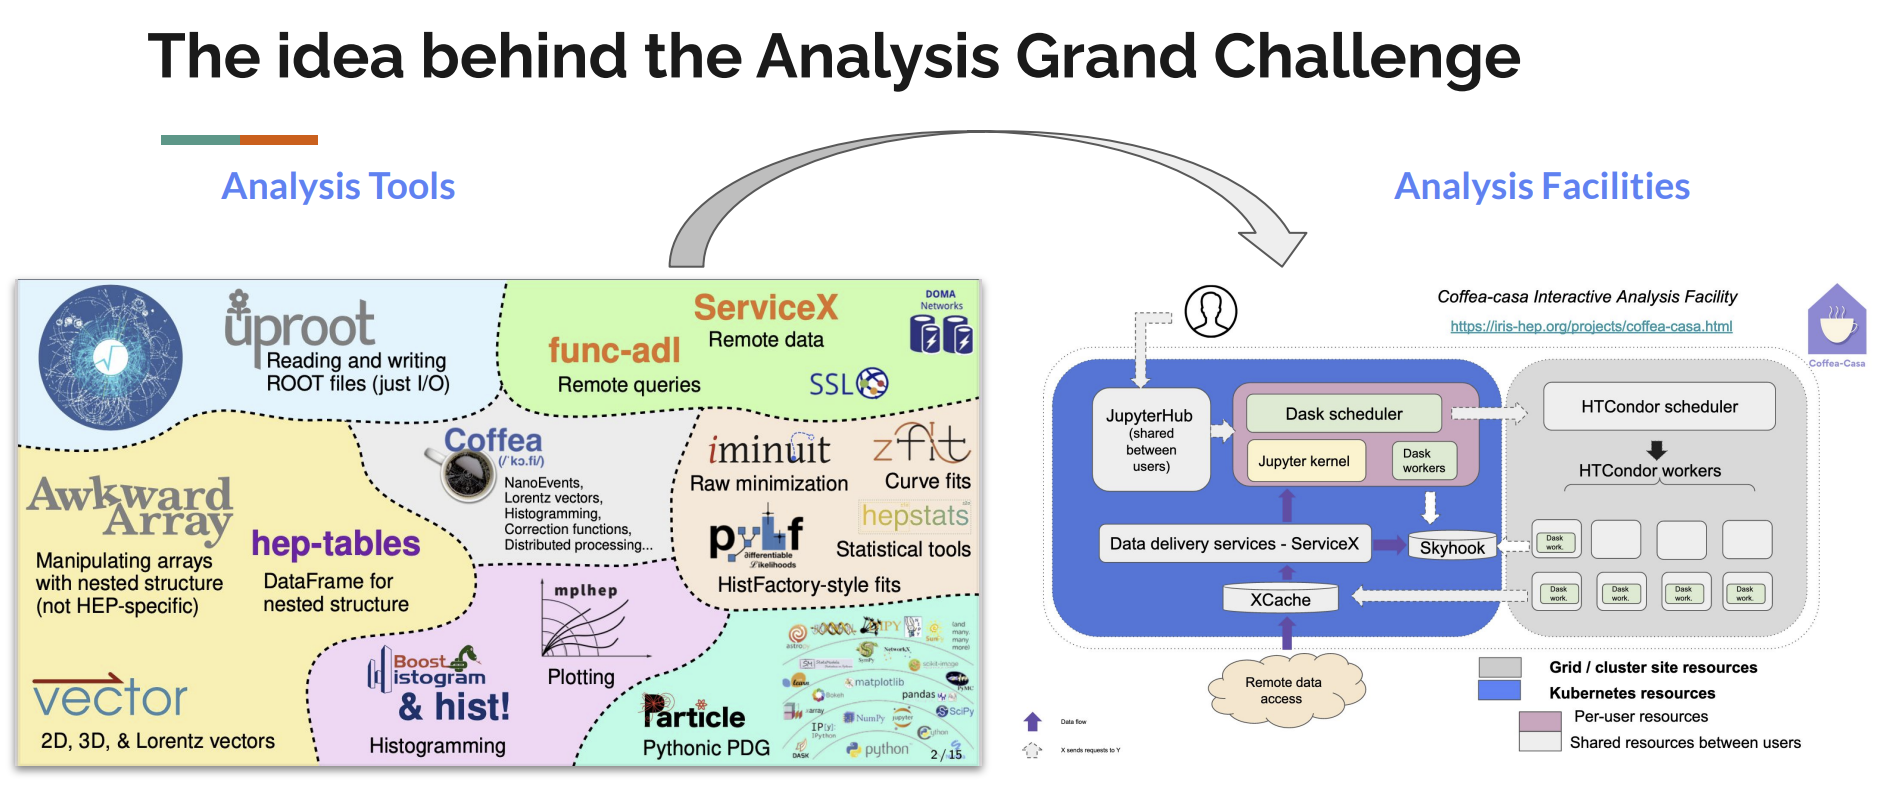
\includegraphics[width=\linewidth]{from-analysis-grand-challenge.png}
\end{columns}
\end{frame}

\begin{frame}{The analysis tools developer community}
\large
{\Large Many people are developing tools\ldots}

\vspace{0.5 cm}
\begin{itemize}\setlength{\itemsep}{0.25 cm}
\item<2-> in IRIS-HEP and out (but mostly communicating on IRIS-HEP's Slack)
\item<3-> each focused on a single purpose, but fitting together into a larger ecosystem
\item<4-> using existing software from beyond HEP whenever possible
\item<5-> mostly in Python
\end{itemize}
\end{frame}

\begin{frame}{Overview of these activities for the LHCC (\href{https://arxiv.org/abs/2202.02194}{arXiv:2202.02194})}
\vspace{0.22 cm}
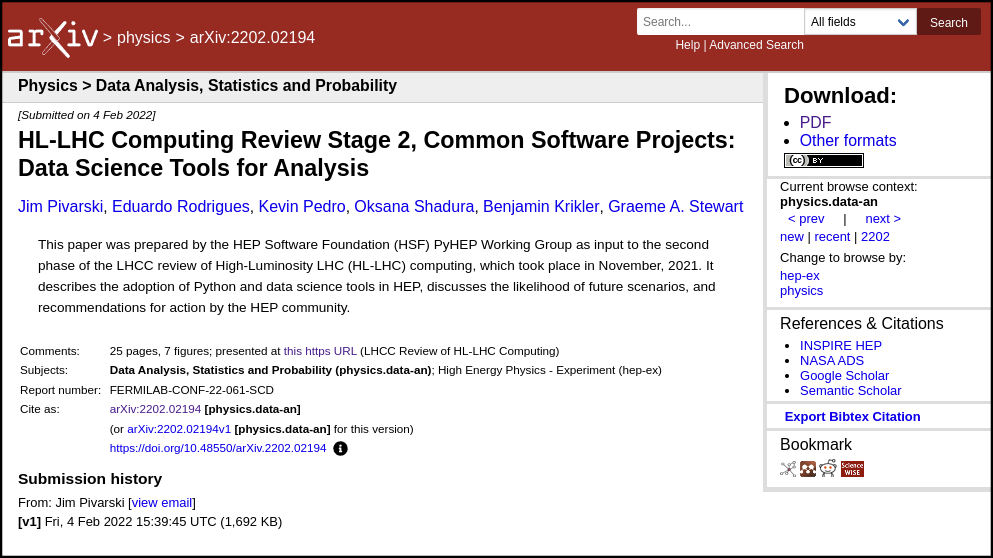
\includegraphics[width=\linewidth]{hl-lhc-data-science-tools-arXiv.png}
\end{frame}

\begin{frame}{\mbox{ }}
\begin{center}
\begin{minipage}{0.85\linewidth}
\large
{\Large A bit different from an ordinary LHC project:}

\vspace{0.25 cm}
\begin{itemize}\setlength{\itemsep}{0.25 cm}
\item The users are distributed (who are they? what do they want?)
\item The developers are distributed (who's working on what?)
\end{itemize}
\end{minipage}
\end{center}
\end{frame}

\begin{frame}{Gathered developers by lighting a beacon: Scikit-HEP}
\vspace{0.18 cm}
\begin{columns}
\column{1.15\linewidth}
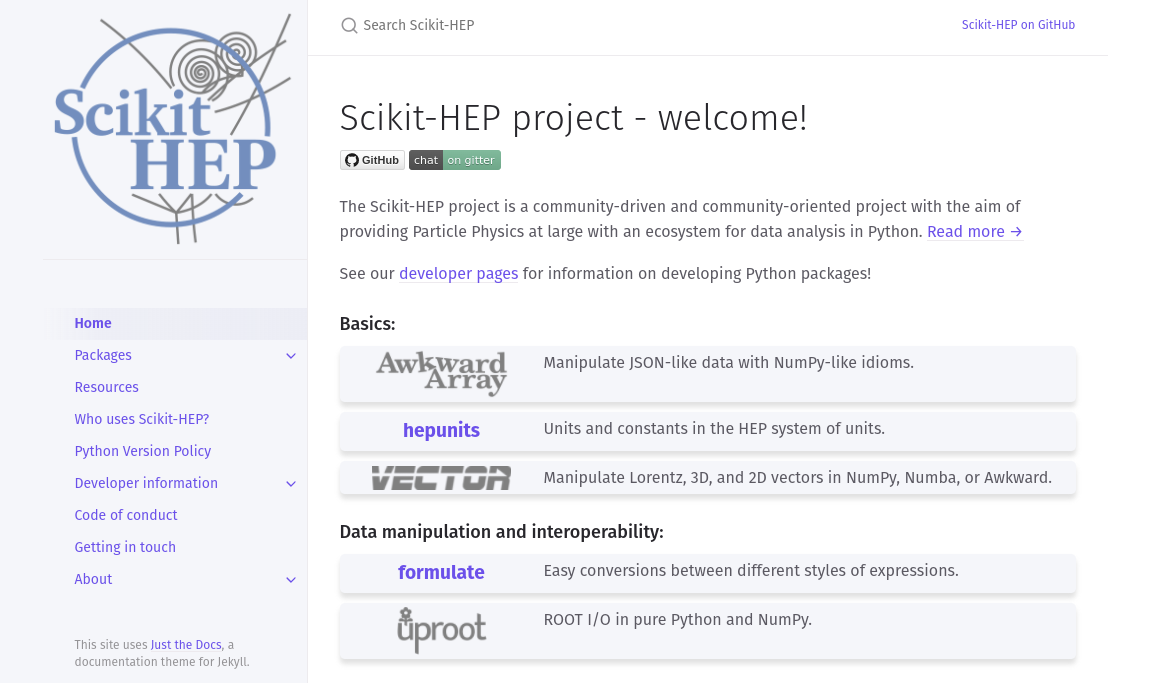
\includegraphics[width=\linewidth]{scikit-hep-webpage.png}
\end{columns}
\end{frame}

\begin{frame}{Stacked download statistics for Scikit-HEP and related projects}
\begin{columns}
\column{1.15\linewidth}
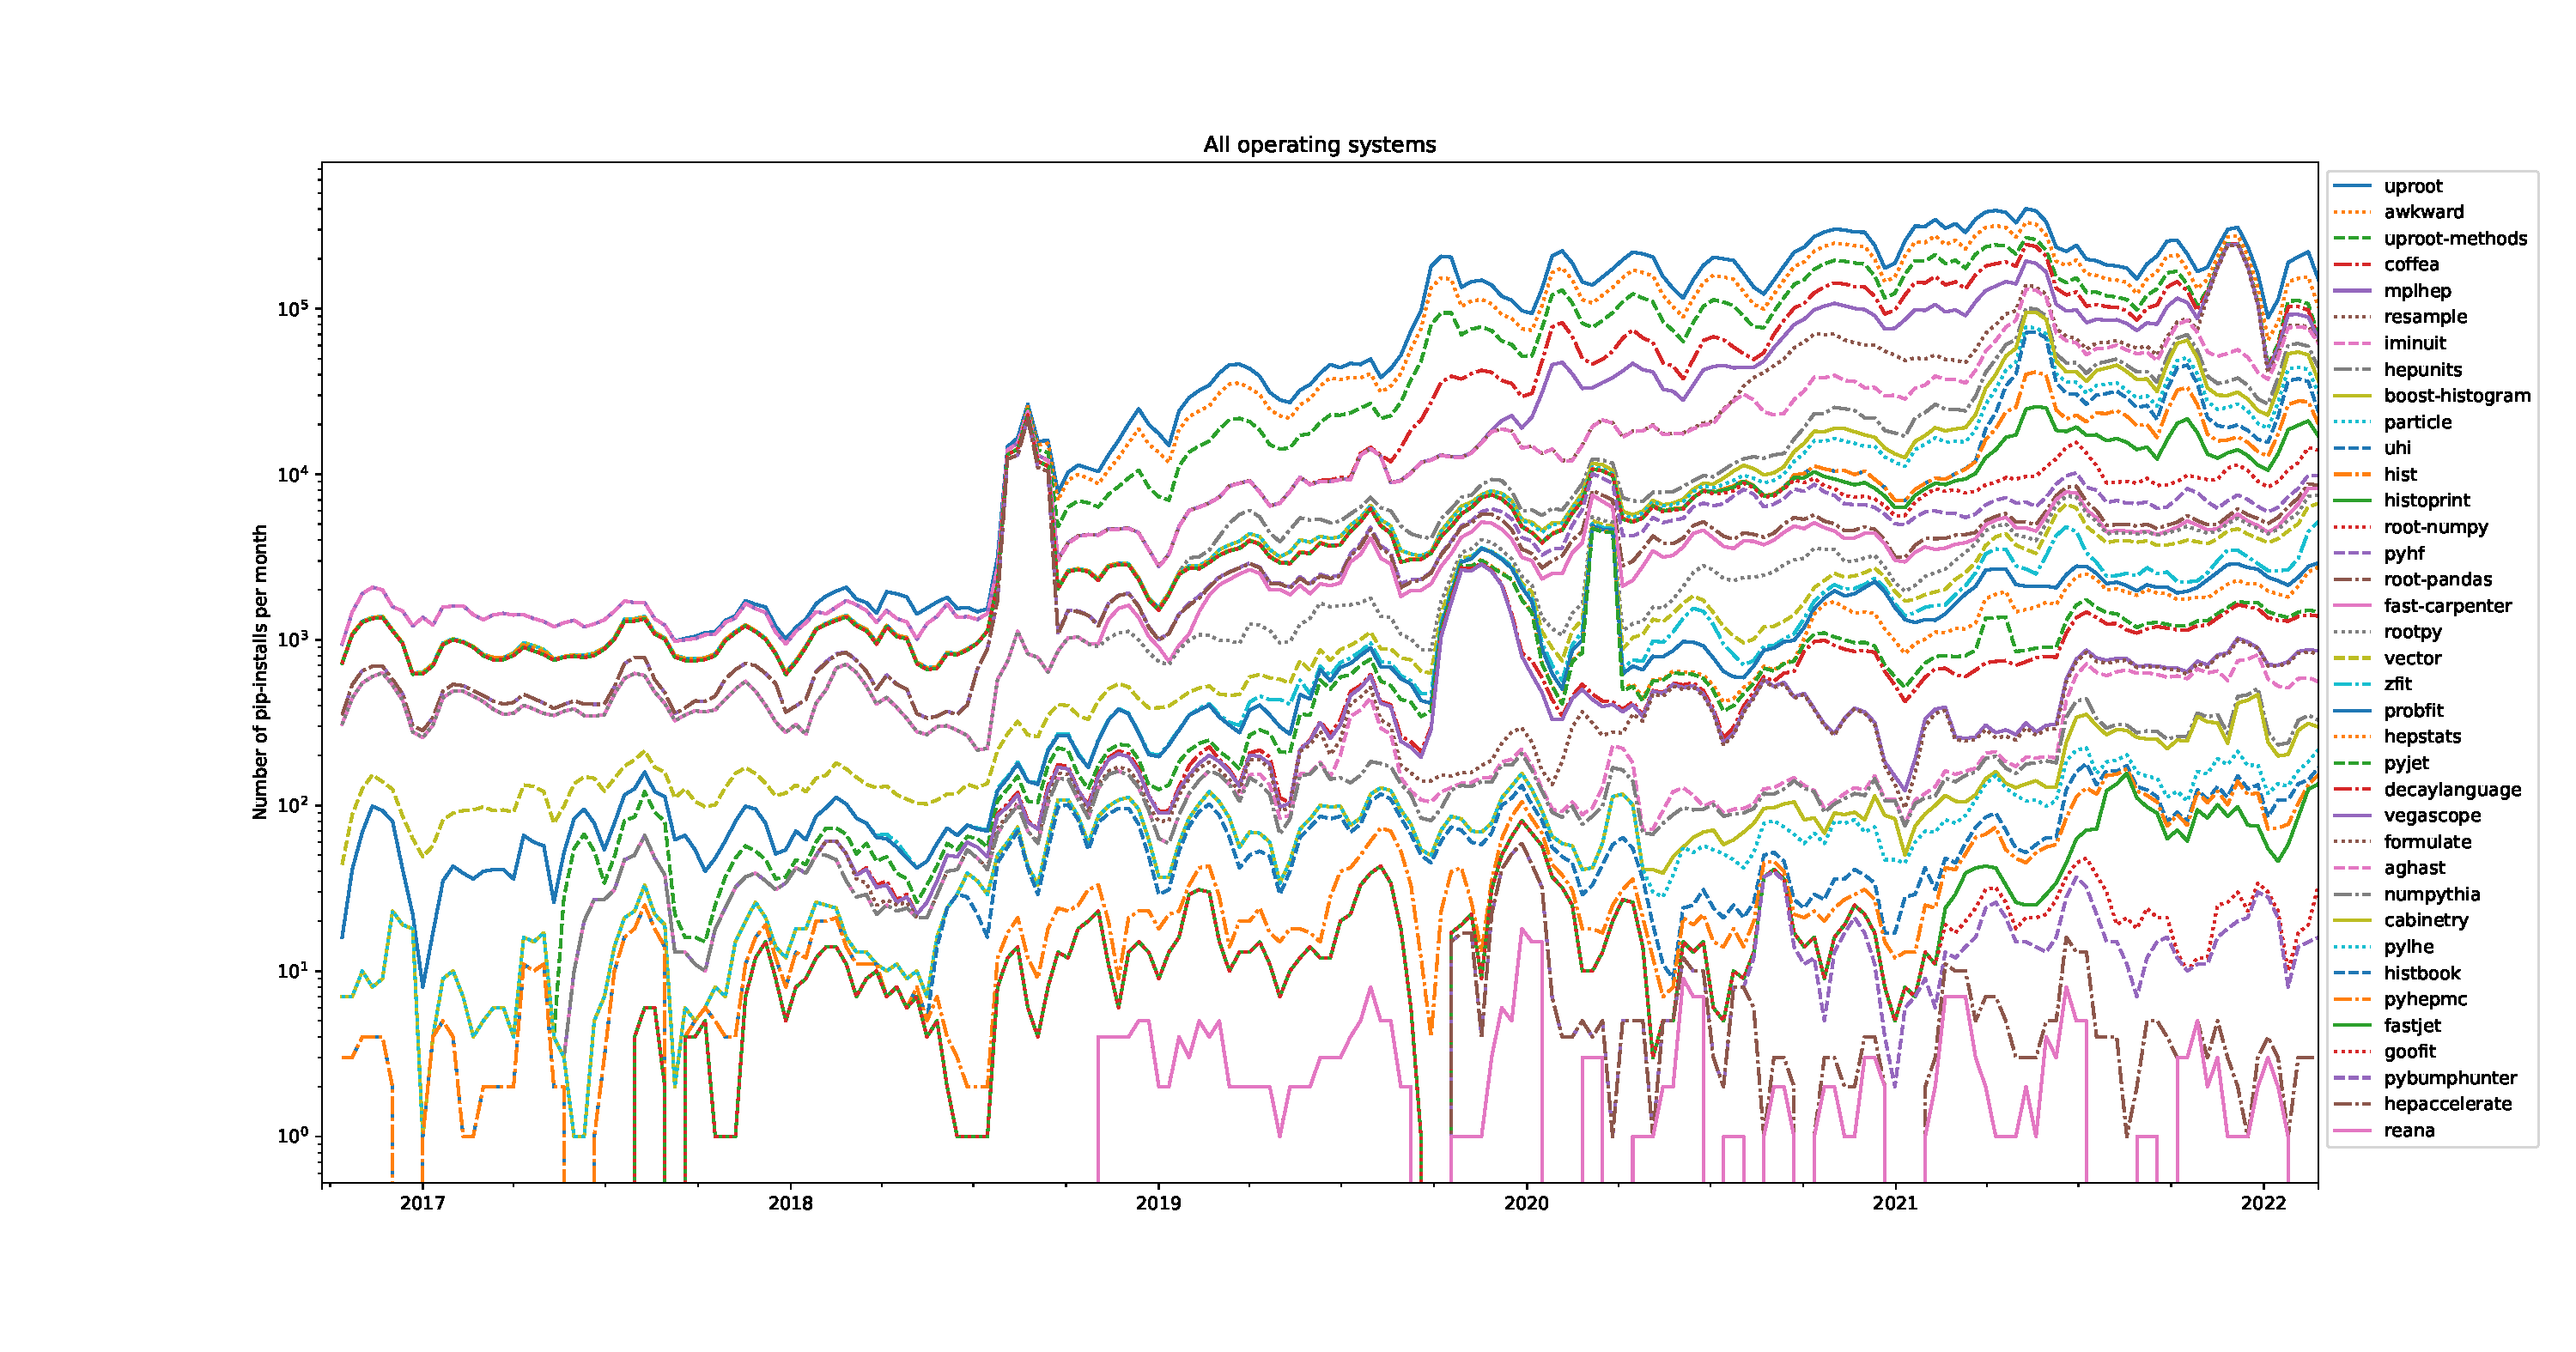
\includegraphics[width=\linewidth]{pip-allos-scikithep-log.pdf}
\end{columns}
\end{frame}

\begin{frame}{Learning about user needs: very different from my expectations!}
\vspace{0.25 cm}
\begin{columns}
\column{1.12\linewidth}
\only<1>{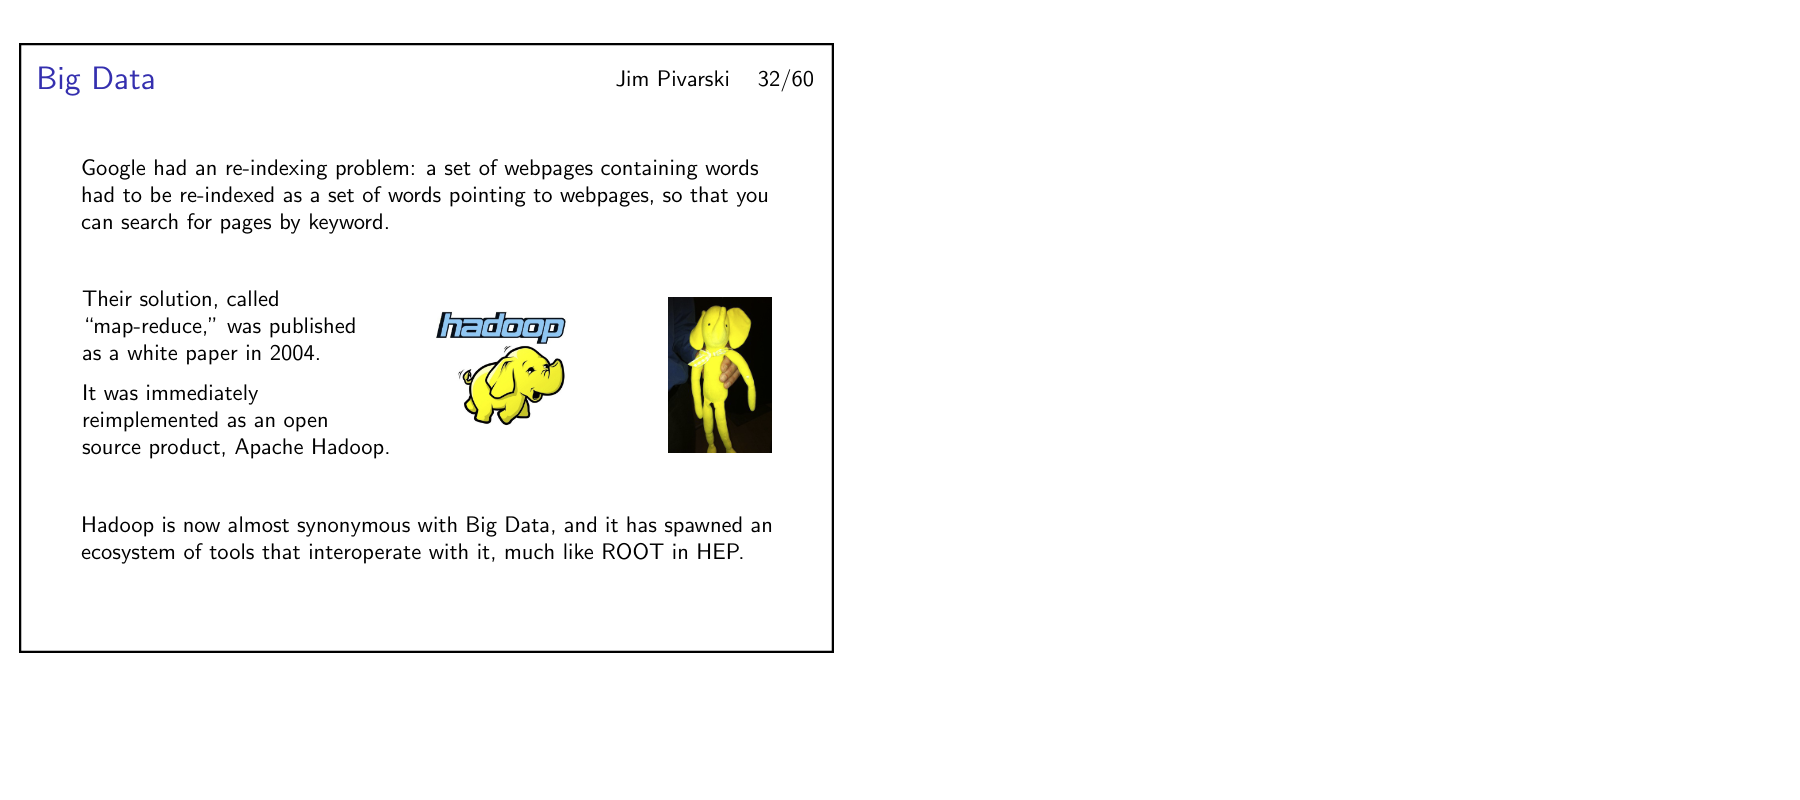
\includegraphics[width=\linewidth]{evolving-views-1.png}}\only<2>{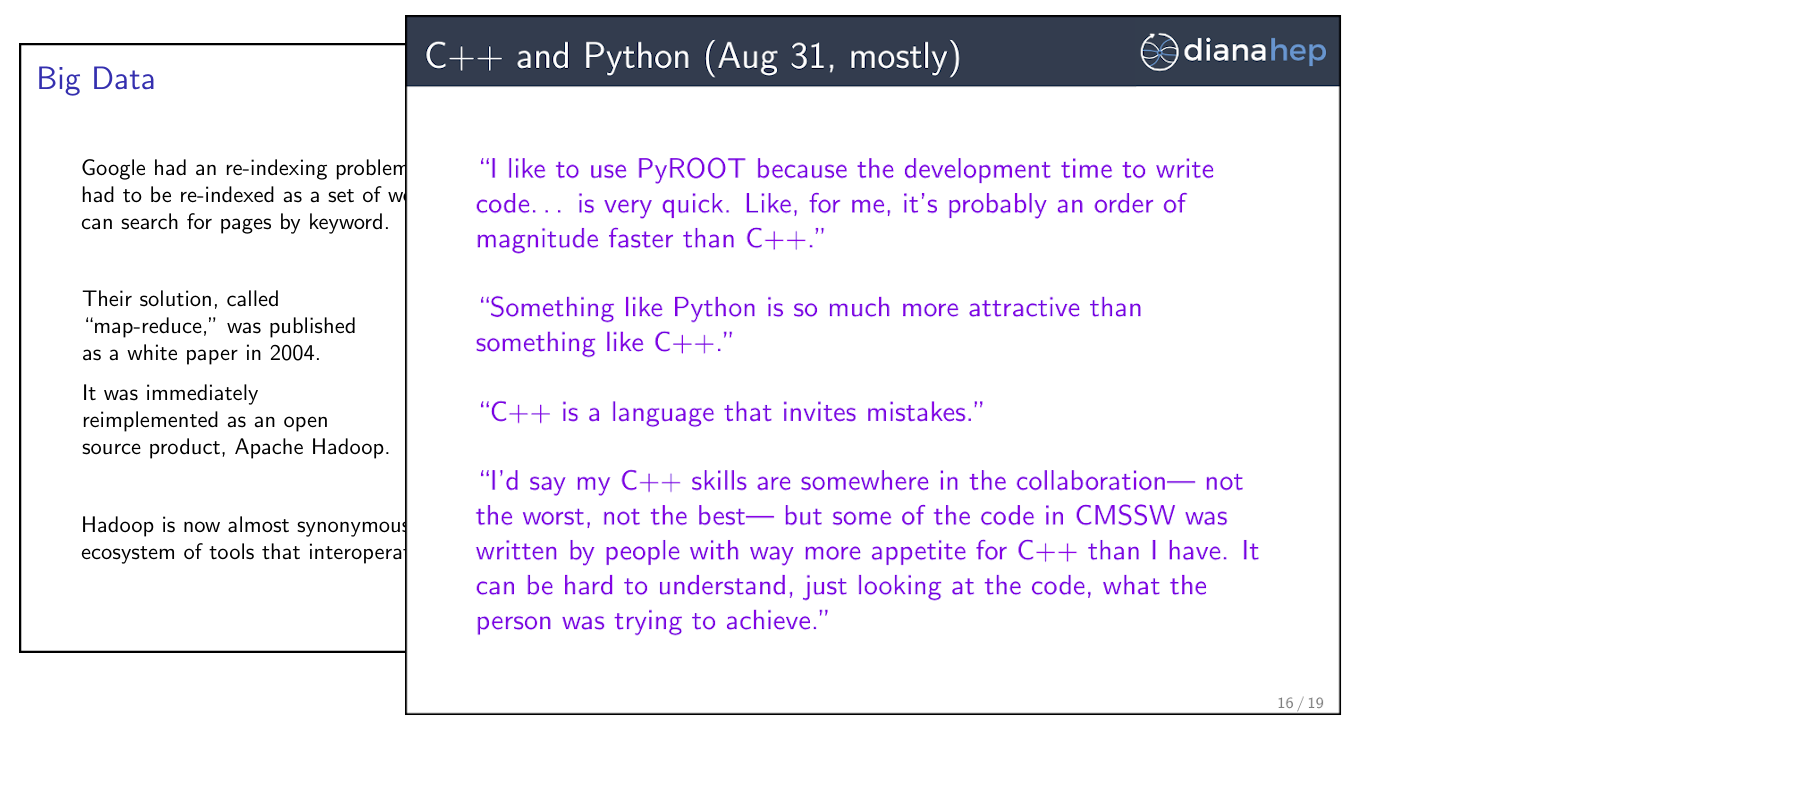
\includegraphics[width=\linewidth]{evolving-views-2.png}}\only<3>{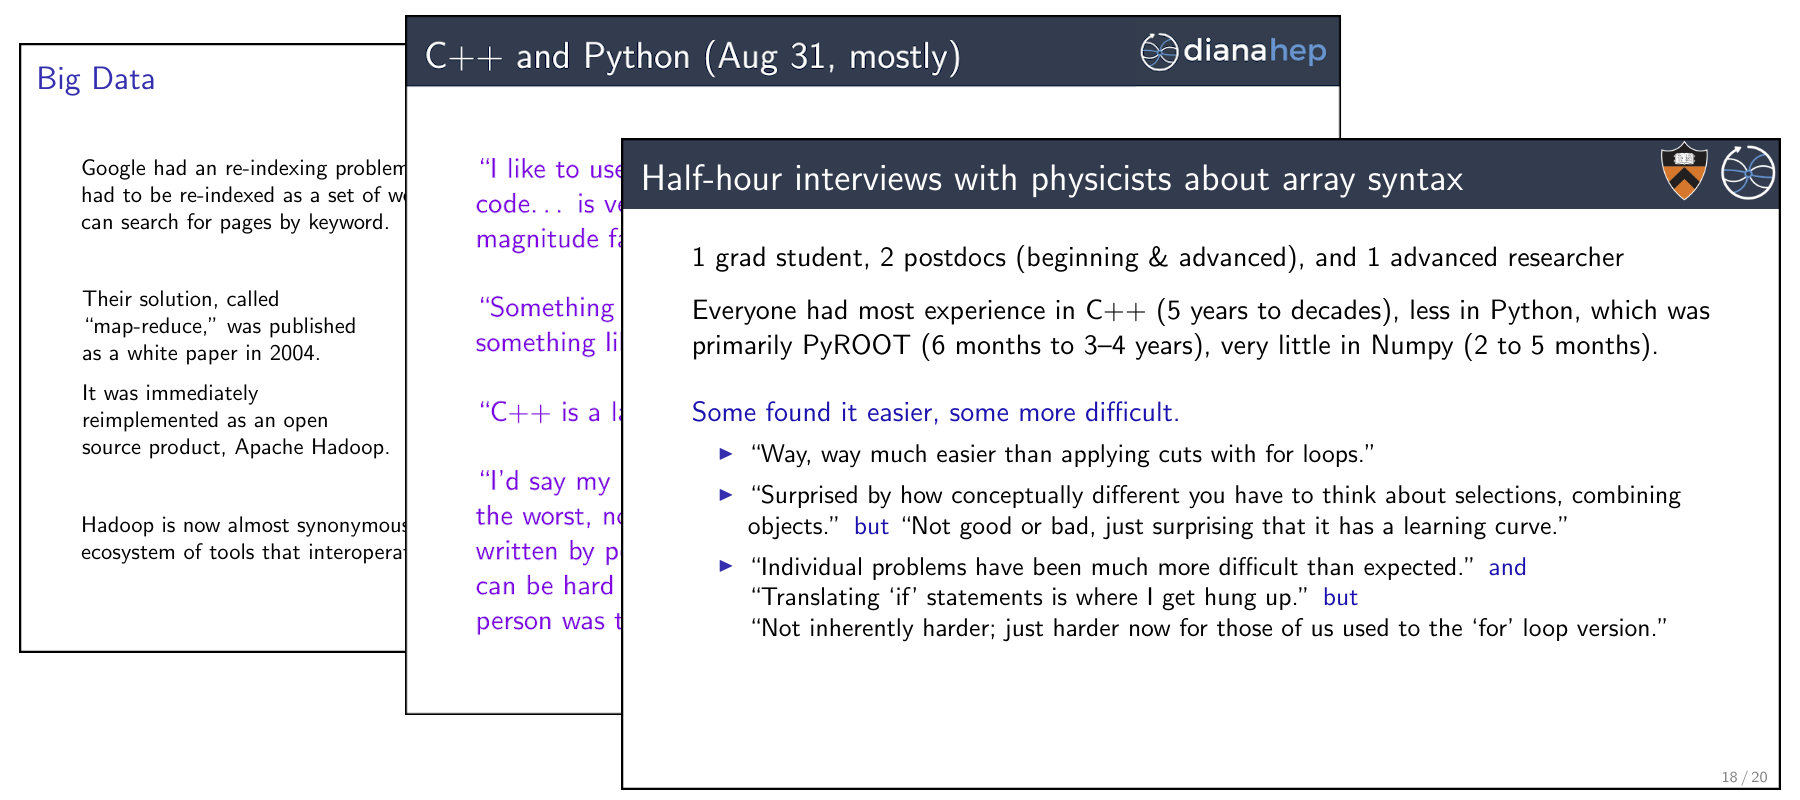
\includegraphics[width=\linewidth]{evolving-views-3.png}}\only<4>{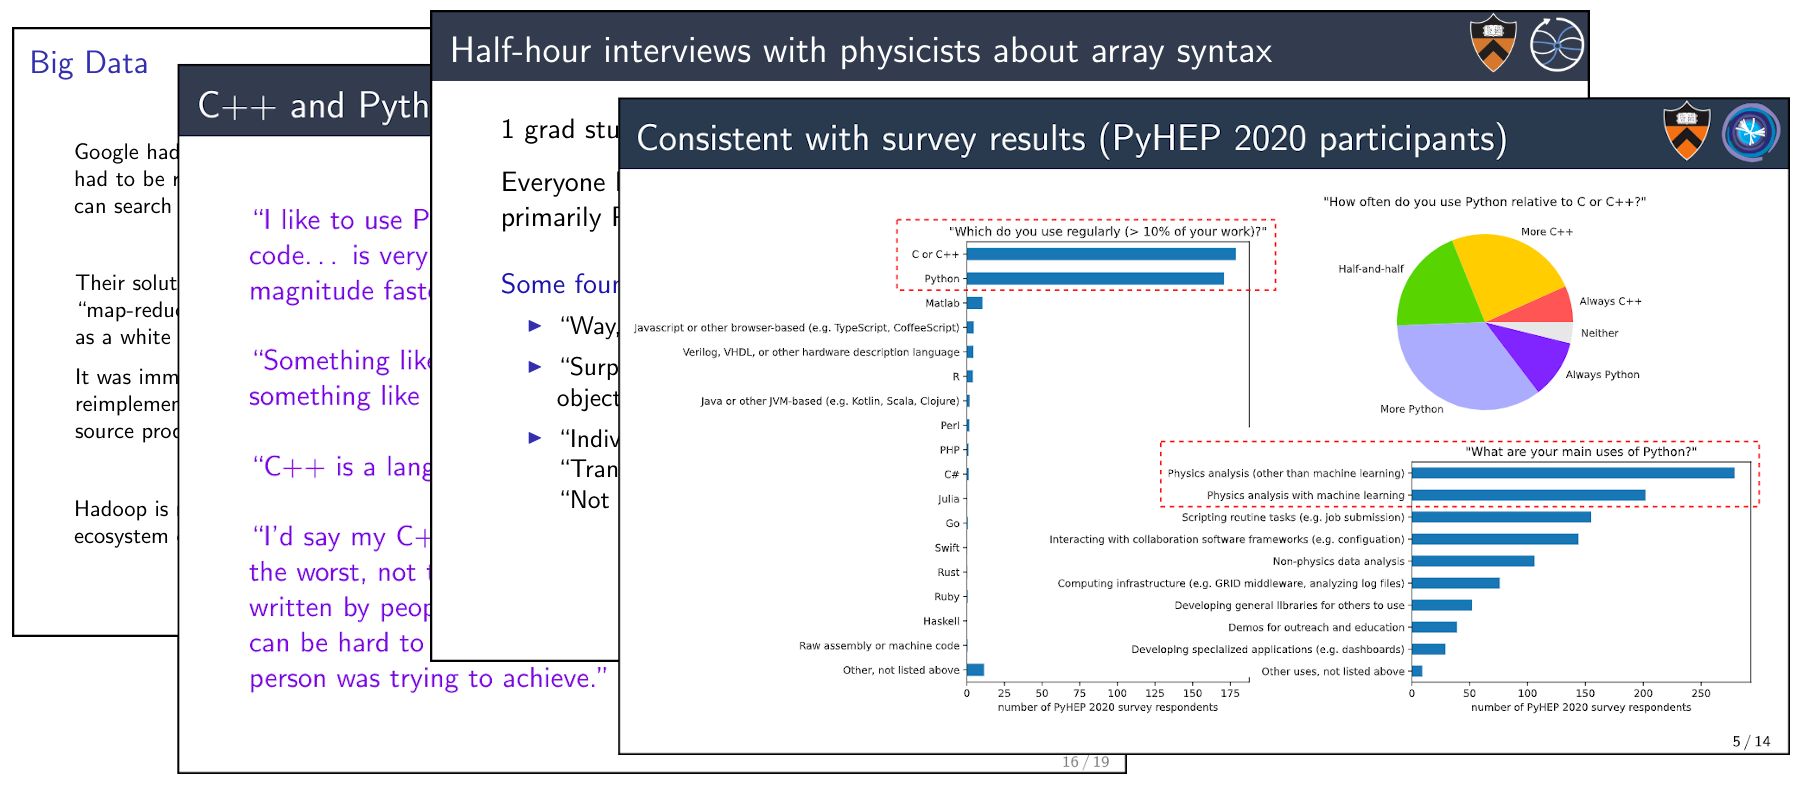
\includegraphics[width=\linewidth]{evolving-views-4.png}}
\end{columns}

\vspace{0.1 cm}
\uncover<2->{\Large\hfill Sought user input in focus groups, interviews, and surveys.}
\end{frame}

\begin{frame}{Small, interoperable Python tools are making a big impact}
\vspace{0.22 cm}
\centering \only<1>{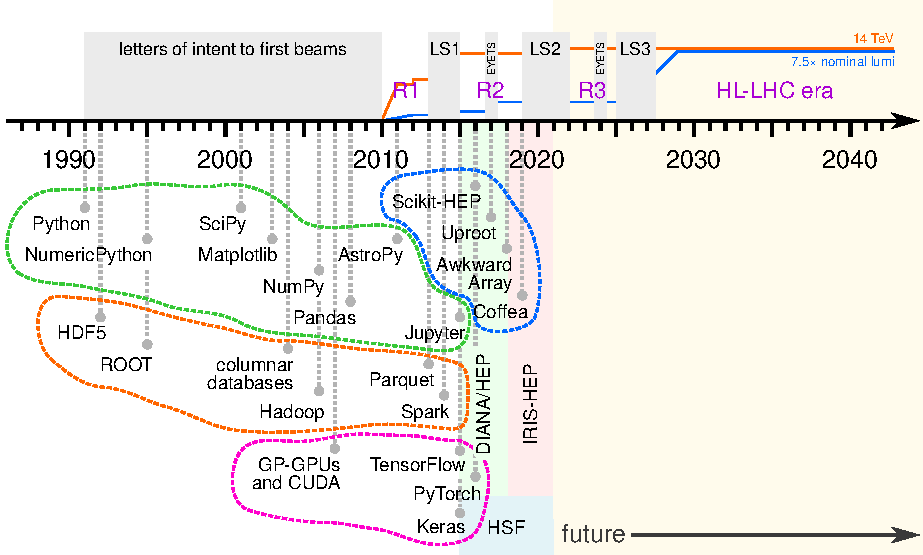
\includegraphics[width=0.92\linewidth]{hllhc-python-timeline-cloud-1.pdf}}\only<2>{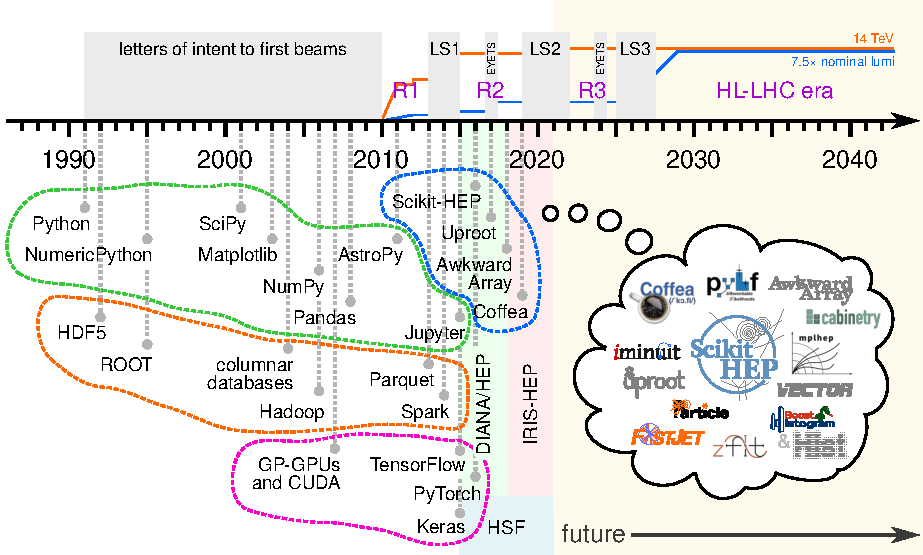
\includegraphics[width=0.92\linewidth]{hllhc-python-timeline-cloud-2.pdf}}
\end{frame}

\begin{frame}{Why Python?}
\large
\vspace{0.25 cm}
\textcolor{darkblue}{\mbox{\hspace{-0.5 cm}}Python is currently leading every ``most popular programming language'' index.}

\vspace{0.25 cm}
\begin{columns}[t]
\column{0.33\linewidth}
\centering Tiobe

\vspace{0.1 cm}
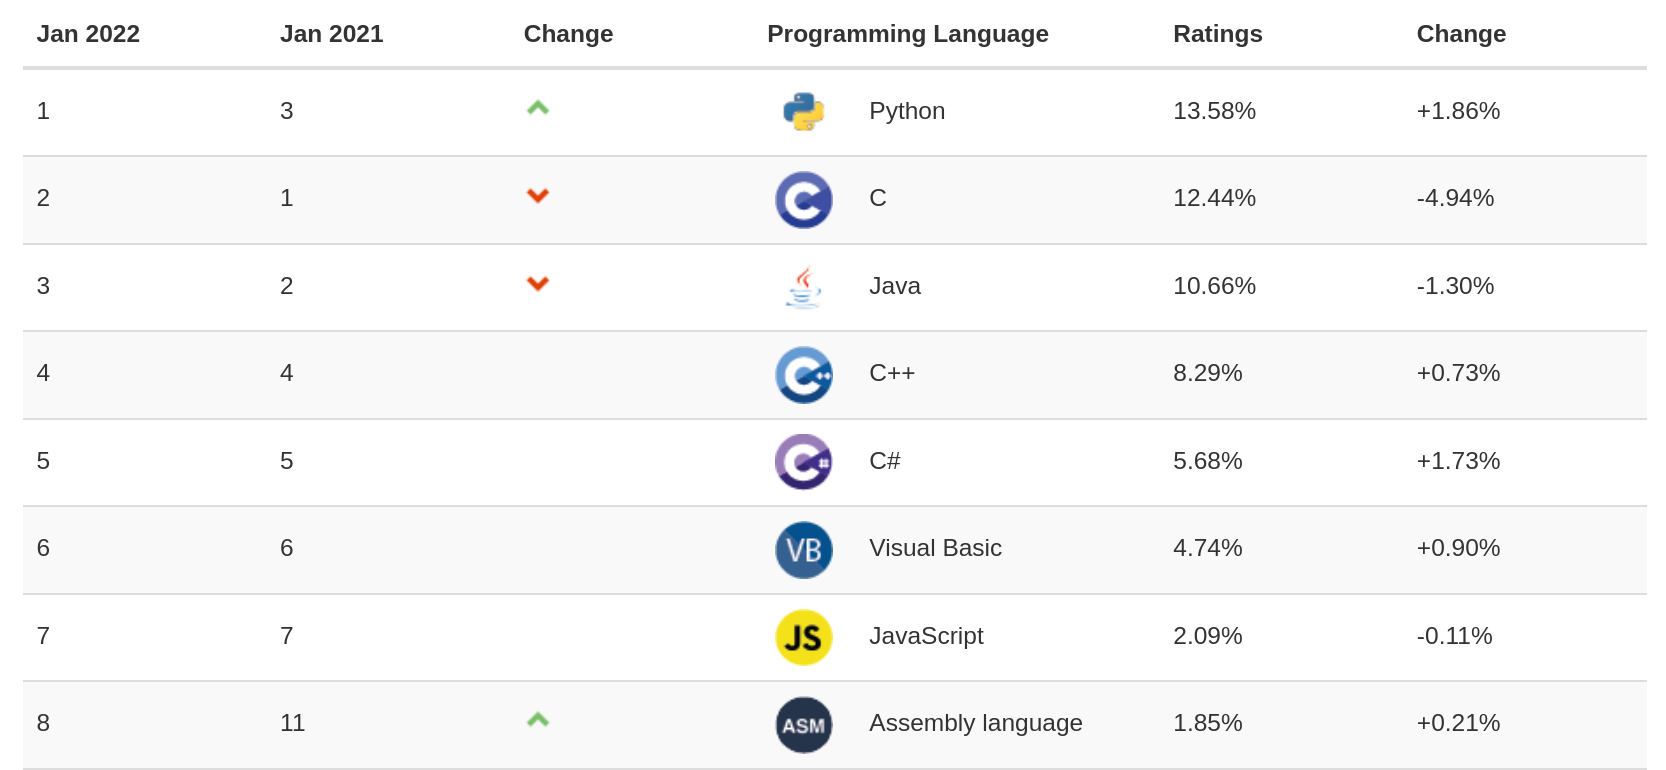
\includegraphics[width=\linewidth]{python-rankings-tiobe-2022.png}

\column{0.33\linewidth}
\centering PYPL

\vspace{0.1 cm}
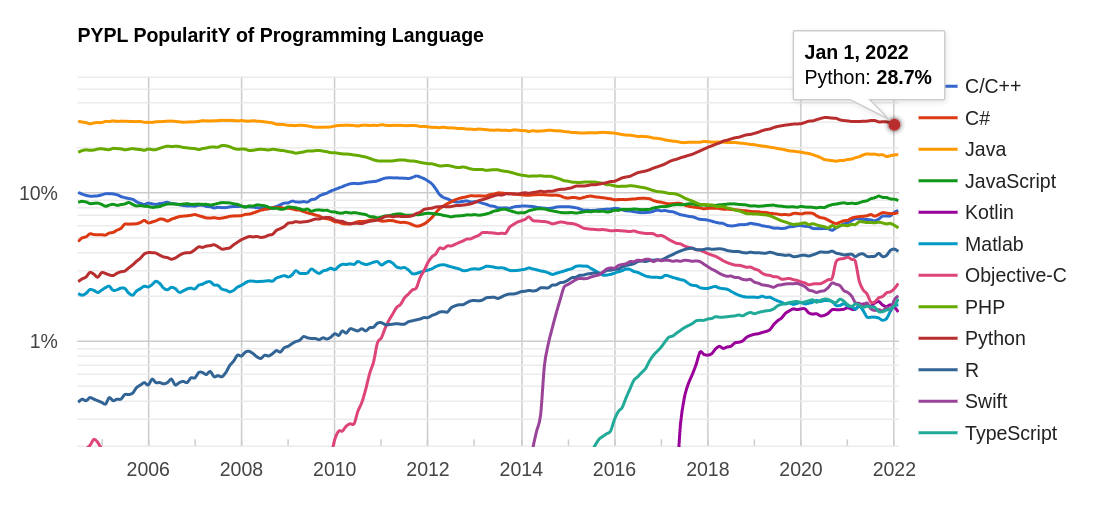
\includegraphics[width=\linewidth]{python-rankings-pypl-2022.png}

\column{0.33\linewidth}
\centering Google Trends

\vspace{0.1 cm}
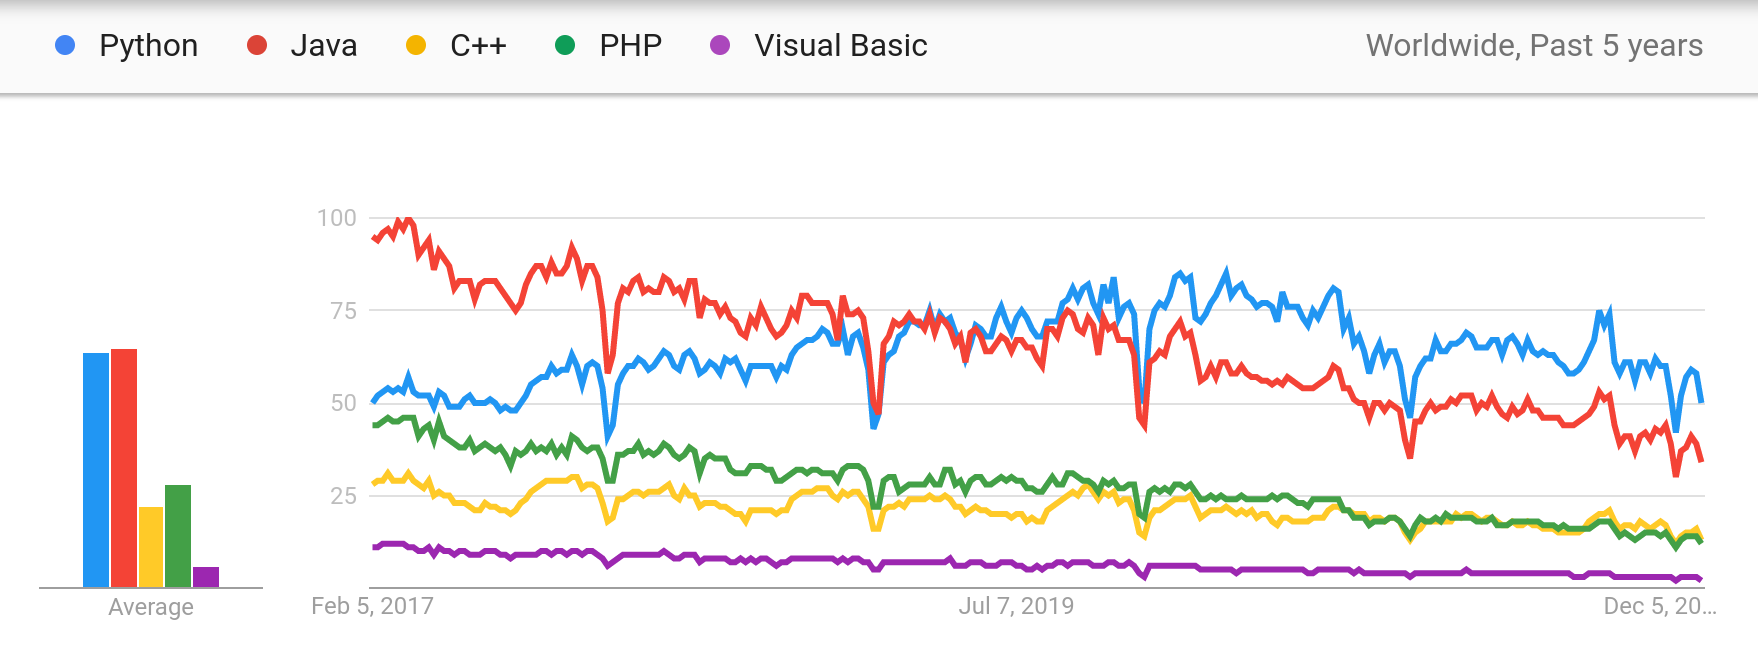
\includegraphics[width=\linewidth]{python-rankings-googletrends-2022.png}
\end{columns}

\vspace{0.25 cm}
\begin{columns}[t]
\column{0.5\linewidth}
\centering GitHut

\vspace{0.1 cm}
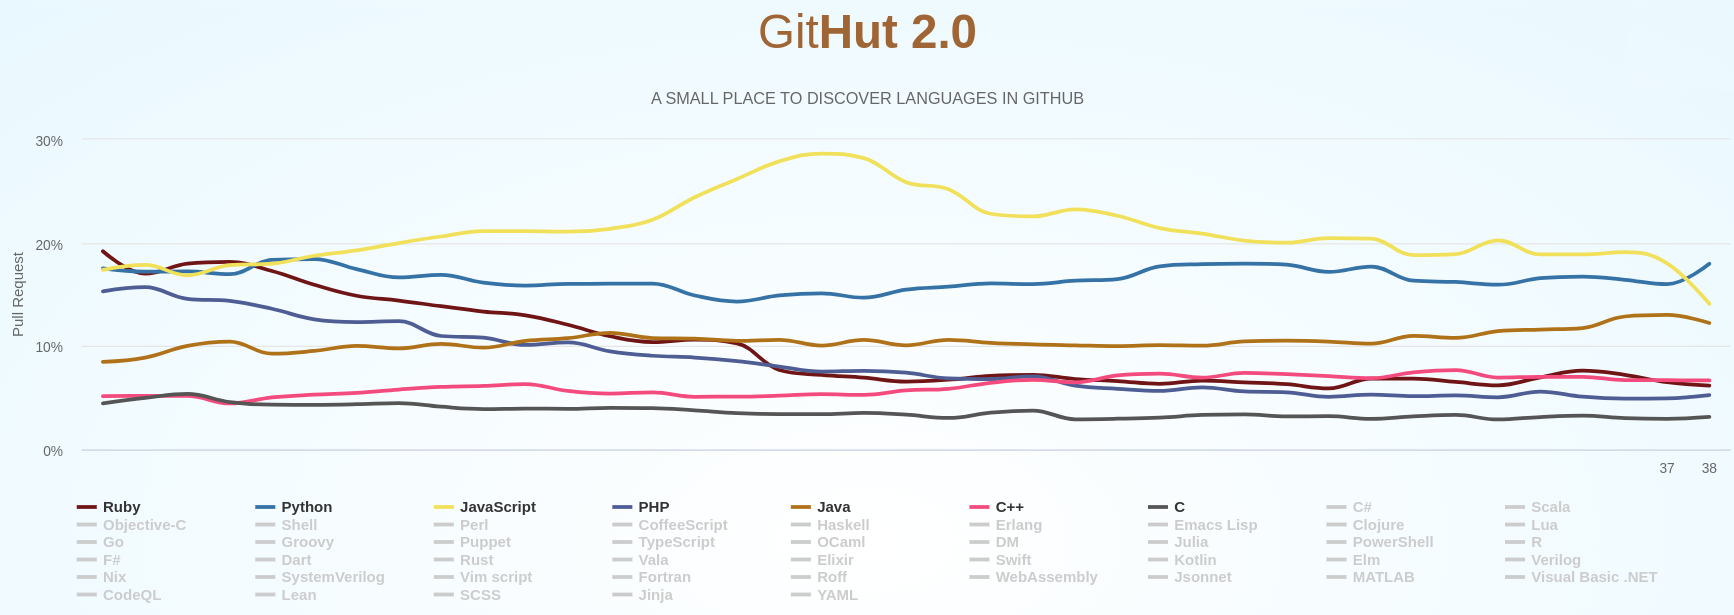
\includegraphics[width=\linewidth]{python-rankings-githut-2022.png}

\column{0.45\linewidth}
\centering StackOverflow

\vspace{0.1 cm}
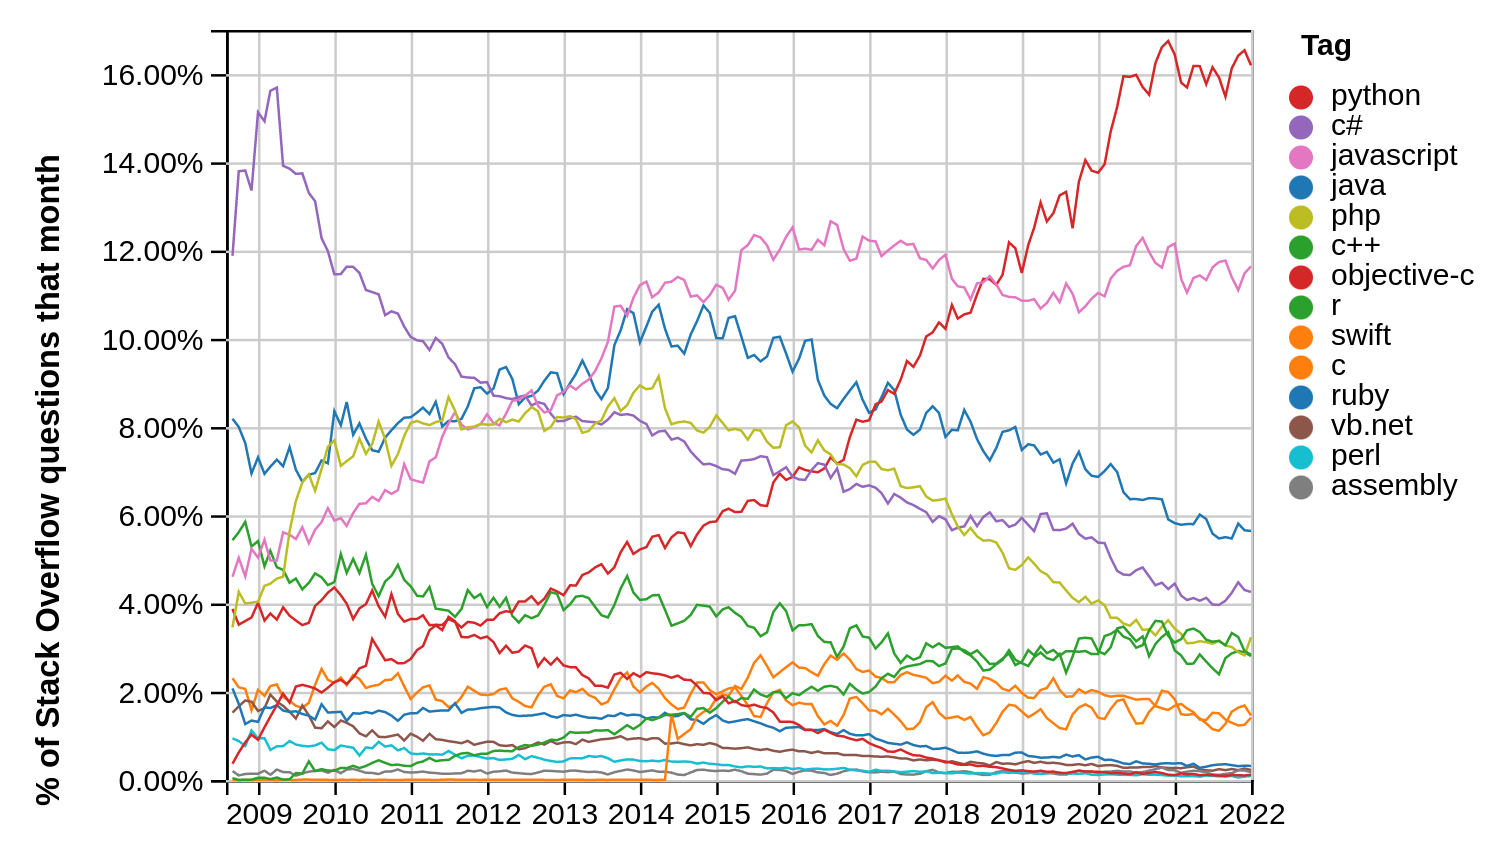
\includegraphics[width=\linewidth]{python-rankings-stackoverflow-2022.png}
\end{columns}
\end{frame}

\begin{frame}{Why Python?}
\large
\vspace{0.25 cm}
\textcolor{darkblue}{\mbox{\hspace{-0.5 cm}}Especially in data analysis. (Below: coincidence of search terms in Google Trends.)}

\vspace{0.15 cm}
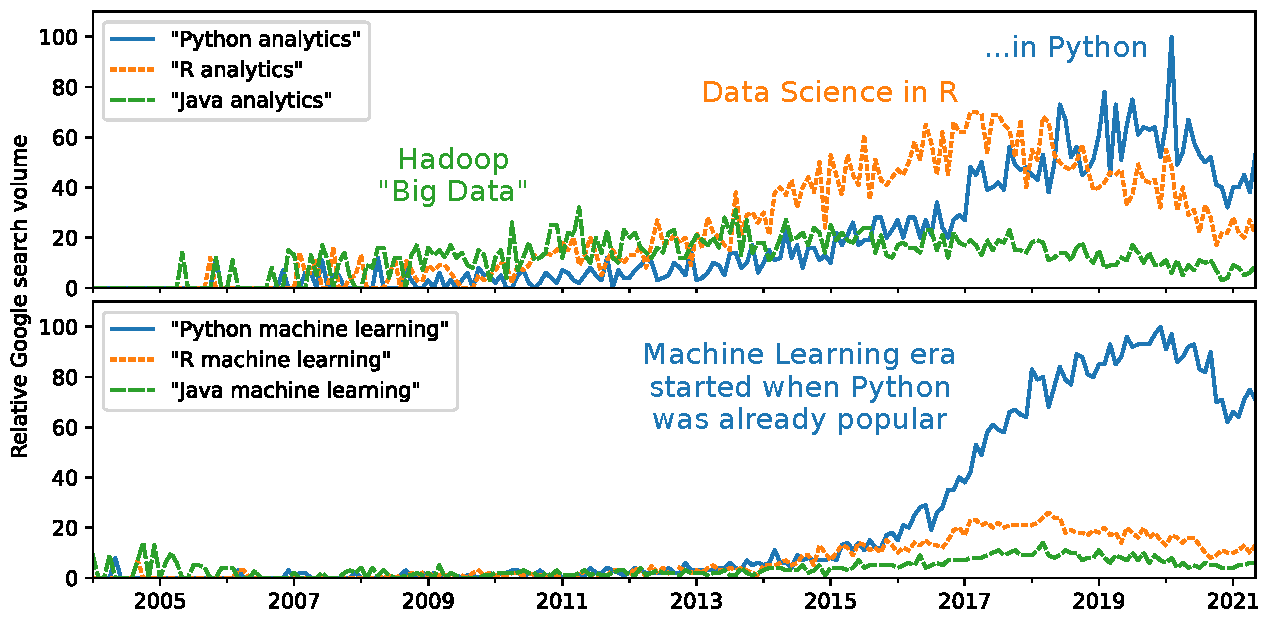
\includegraphics[width=\linewidth]{analytics-by-language.pdf}
\end{frame}






%% \begin{frame}{\mbox{ }}
%% \Large
%% \begin{center}
%% Software for the HL-LHC is usable today: get feedback today.

%% \vspace{1 cm}
%% Gives us the flexibility to follow unexpected changes in direction.

%% \vspace{1 cm}
%% Small pieces can be ``swapped out'' as we learn more.
%% \end{center}
%% \end{frame}




\end{document}
